\chapter{Logic Gates in Neural Networks}\label{ch_logicgates}
\chapterauthor{Jeff Yoshimi}

% Say more about relation to computers. Languages are compiled down to machine language which operates on bits and the computers ultimately just use these kinds of operations.
% See Fausett section 1.6

We opened the book by noting that neural networks are very different from classical computers. They are trained, not programmed, they transform data using weight matrices rather than explicit rules, they gracefully degrade and do well with noisy inputs. We made the contrast by comparing neural networks with Turing Machines, a simple type of machine that captures the kinds of things classical computers do. One thing classical computers do is simple logical computations.In fact, all the incredible things computers do can be boiled down to a bunch of simple logical computations. \textbf{Logic gates} are fundamental components of the circuits that make up digital computers. If a neural network could do the same thing, it would show that neural networks could, at least in principle, do anything a digital computer could do.

This problem occupied McCulloch and Pitts, the early pioneers of neural networks: how to make neural networks do logical computations, and implement logic gates. It turns out, they can do this  (and thus, neural networks are as powerful as digital computers!) \cite{mcculloch1943logical}. Understanding these logic functions and how neural networks can compute them is the goal of this section.

We will consider 4 kinds of logic gate: NOT, AND, OR, and XOR. We can think of these in logical terms, as \textbf{boolean functions}. These functions take truth values as inputs, and produce other truth values as outputs. Here is roughly how these four boolean functions work:

\begin{itemize}
\item NOT P is True if P is false.
\item P AND Q is True if both P and Q are True.
\item P OR Q is True if P is True, Q is True, or both P and Q are True.
\item P XOR Q is true if one of P or Q is True, but not both.
\end{itemize}

To implement these on a neural network (and see in more detail how they work), we  can map True to the number 1 and False to the number 0, and then think of these as vector-valued functions that take vectors of binary values as inputs and produce a single 0 or 1 as an output. It is standard in logic to represent boolean functions with \textbf{truth tables}, which are basically the tables we have been using to represent vector-valued functions in neural networks. Here is a truth table which represents the logic of AND:

\begin{center}
\begin{tabular}{| c | c || c | }
\hline
  P  & Q & P AND Q  \\
\hline
  1 (T) & 1 (T) & 1 (T)  \\
\hline
 1 (T) & 0 (F) & 0 (F)  \\
\hline
 0 (F) & 1(T) & 0  (F) \\
\hline
 0 (F) & 0 (F) & 0 (F) \\
\hline
\end{tabular}
\end{center}

In this table,  P and Q can be interpreted as the truth values of sentences. We can replace P and Q with any sentence that can be true or false. For example P could stand for ``I ate pizza'' and Q could stand for ``I drank soda.''  The four rows of the table then show all possible combinations of truth values for these two statements. It could be that I didn't eat  pizza or drink soda (row 4), that I drank soda and ate pizza (row 1), that I only ate pizza (row 2), etc. The third column shows us the output of the boolean function for each of these combinations of truth values. For example, focusing on row 1: if I did eat pizza (P) and drink soda (Q), then it's also true that I ate pizza and drank soda (P AND Q). 

NOT is also a boolean function, from one input to one output, that basically reverses the truth value of the input when it produces its output:

\begin{center}
\begin{tabular}{| c || c | }
\hline
  P  & NOT P  \\
\hline
  1 (T) & 0 (F)  \\
\hline
 0 (F) & 1 (T)  \\
\hline
\end{tabular}
\end{center}

%This can be thought of as a vector-valued function from vectors in a 2-d space to vectors in a 1-d space.

Here is a combined truth table showing several other two-valued boolean functions as extra columns, including OR and XOR. XOR is ``exclusive'' or, which is only true if exactly one of P and Q is true. OR is ``inclusive'' or, which is true when one or both of P and Q is true.

\begin{center}
\begin{tabular}{| c | c || c || c || c | }
\hline
  P  & Q & P AND Q  & P OR Q & P XOR Q \\
\hline
  1 (T) & 1 (T) & 1 (T) & 1 (T) & 0 (F) \\
\hline
  1 (T) & 0 (F) & 0 (F) & 1 (T) & 1 (T) \\
\hline
  0 (F) & 1 (T) & 0 (F) & 1 (T) & 1 (T) \\
\hline
 0 (F) & 0 (F) & 0 (F) & 0 (F) & 0 (F) \\
\hline
\end{tabular}
\end{center}

We can implement any of these functions in a neural network. The input layers will have two nodes, and the output layer will have one node. For example, a network to compute AND would only produce an output of 1 if both input nodes were set to 1. In all other cases of binary inputs the output would be 0. Using binary output functions and appropriate weights and thresholds, it is not so hard to make AND and OR gates. 

NOT would just have two nodes. A 0 would produce a 1 and a 1 would produce a 0. This can be done using a binary output node with a bias (so that it is on, by default, above threshold), and a negative weight.

XOR is harder because it requires a few layers of nodes (a point that is important when we talk about supervised learning), but basically it involves combining an OR gate to the output and an intermediate AND gate that inhibits the output. Examples of these are shown in Fig. \ref{logic_gates}.

\begin{figure}[h]
\centering
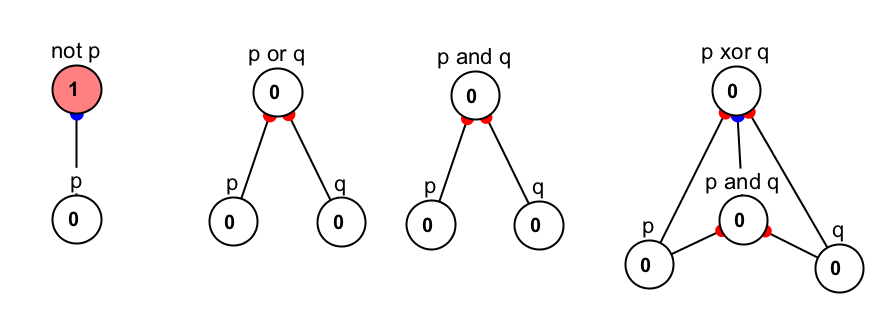
\includegraphics[scale=.7]{./images/logic_gates.png}
\caption[Simbrain screenshot]{Networks to implement basic logic gates.}
\label{logic_gates}
\end{figure}

Boolean functions can also be combined, to produce things like (P AND (Q OR NOT R)). To see what the truth table looks like for this type of network, you can try an online resource like \url{http://web.stanford.edu/class/cs103/tools/truth-table-tool/}. Neural networks to implement this type of function are also not too difficult to make, by combining together the other networks, e.g the output of an OR network is one of the two inputs to the AND network, to make (P AND (Q OR NOT R)).

A complex example, in which sample sentences have been used instead of the boring propositional variables P, Q, R etc., is shown in Fig. \ref{logic_gates_ex}.

\begin{figure}[h]
\centering
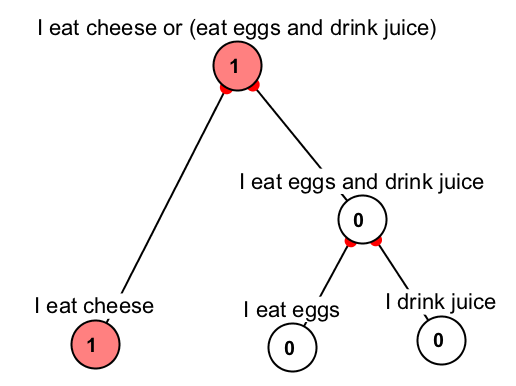
\includegraphics[width=0.4\textwidth]{images/logic_gates_ex.png}
\caption[Simbrain screenshot]{Network to implement a more complex boolean function.}
\label{logic_gates_ex}
\end{figure}

